\section{Ensemble Methods}
Ziel: Mehrere Modelle zu nutzen um ein Problem zu lösen. Anstelle das perfekte Modell zu nutzen, werden mehrere (schlechtere) Modelle trainiert und die Ergebnisse aggregiert.\\
\textbf{Wisdom of Crowd}: Bei einer komplexen Frage mehrere zufällig ausgewählte Personen fragen und Ergebnisse aggregieren. Dies funktioniert wahrscheinlich sehr gut und ist auch einfacher als die am besten passende Person, den Experten zu finden. Dieses Konzept kann mit Ensemble auf Machine Learning übertragen werden. Wir erhalten je nach dem sogar ein viel besseres Resultat als mit nur einem Modell. Ensemble steht für «A group of Predictors», «Ensemble Learning», «Ensemble Method» Ensemble Methoden werden meist gegen ende eines Projekt benötigt, wenn man bereits einige gute Predictors hat und diese kombinieren will.
\subsection{Unterschiedliche Dimensionen}
\textcolor{myblue}{Unterschiedliche Algorithmen}\\
Wir kennen beispielsweise zwei Methoden für die Klassifizierung. Diese können wir kombinieren. Z.B. KNN und Logistic Regression.
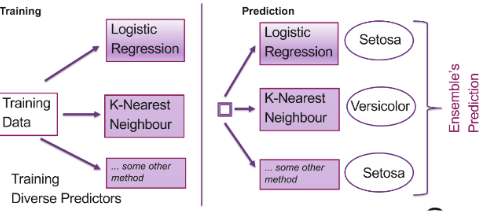
\includegraphics[width=\linewidth]{img/diverse_predictors.png}
\textcolor{myblue}{Unterschiedliche Hyperparameter}\\
Wir können bei KNN verschiedene k verwenden. Oder bei Logistic Regression diverse Regularisierungsparameter.\\
\textcolor{myblue}{Unterschiedliche Trainingsdaten}\\
Wir können Cross Validation Nutzen und dann die Ergebnissie kombinieren oder diverse Features aus Feature Engineering kombinieren. So haben wir unterschiedliche Splits.
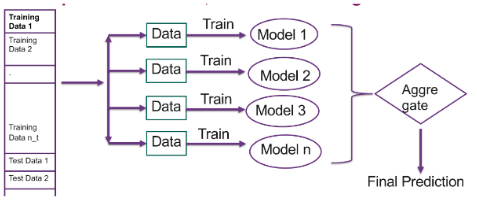
\includegraphics[width=\linewidth]{img/diverse_training_data.png}
\subsection{Voting}
\textcolor{myblue}{Hard}\\
Beim harten Voting wird die Klasse genommen mit den meisten Votes. Beispiel in der Grafik oben wird Setosa genommen, da
dies zwei mal vorkommt und Versicolor nur einmal.\\
\textcolor{myblue}{Soft}\\
Kann nur genommen werden, wenn Ergebnisse Warscheinlichkeiten sind, nicht Klassen. Dann kann man einen Durschnitt aus
allen Modellen nehmen.
\subsection{Auswählen der Daten (Bagging)}
Für die verschiedenen Modelle müssen die Daten aufgesplittet werden. Da gibt es grob zwei Varianten:\\
\textbf{Sampling without Replacement:} Datenpunkt kann nur einmal selektiert werden. -> Pasting
\textbf{Sampling with Replacement:} Datenpunkt kann mehrmals selektiert werden. -> Bagging (Bootstrap Aggregating)
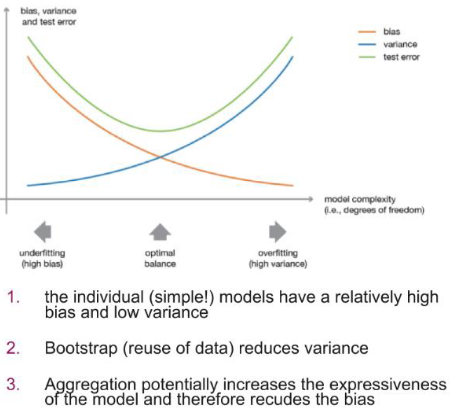
\includegraphics[width=\linewidth]{img/choose_data.png}
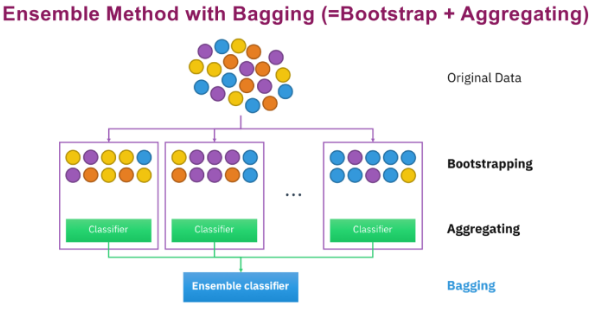
\includegraphics[width=\linewidth]{img/ensemble_method_bagging.png}
Bagging kann auch für Features gemacht werden nicht nur für die Daten. So kriegt man noch mehr unterschiedliche Modelle. (max\_features und bootstrap\_features).\\
Sampling both features and training data -> Random Patches\\
Sampling only features -> Random Subspace\\
\subsection{Out of Bag (oob) Evaluation}
Es gibt Datenpunkte die nie gewählt werden wenn man die Datenpunkte zufällig wählt. Dies sind dann oob-Punkte. Diese können genutzt werden als Testdaten um das Modell zu trainieren. So braucht man nicht extra vorher die Daten aufzuteilen in Trainings- und Testdaten.
\subsection{No free lunch theorem}
Warum Ensemble statt alle Zeit investieren in die Optimierung eines einzelnen Modells? Antwort: Weil kein einzelner Algorithmus die Lösung ist für ein Problem und es keinen besten Algorithmus gibt. Wichtige Punkte die zu beachten sind:
\begin{itemize}
\item Kein einzelner Algorithmus kann alle Probleme besser lösen als jeder anderer Algorithmus
\item Machine Learning muss richtig verstanden werden, genauso die involvierten Daten, bevor man den Algorithmus wählt
\item Jedes Modell ist nur so gut, wie die Daten die wir haben und den Schlüssen, die man daraus zieht.
\item Einfachere Modelle, wie Logistic Regression, tendieren eher dazu zu underfitten und haben mehr Bias. Zu komplexe Modelle führen zu grösseren Varianzen und tendieren zum Overfitting.
\item Die besten Modelle sind jeweils in der Mitte von zwei Bias-Varianzen-Extremen
\item Um ein gutes Modell zu finden, muss man mehrere unterschiedliche Modelle probieren und vergleichen mittels Cross-Validation.
\end{itemize}
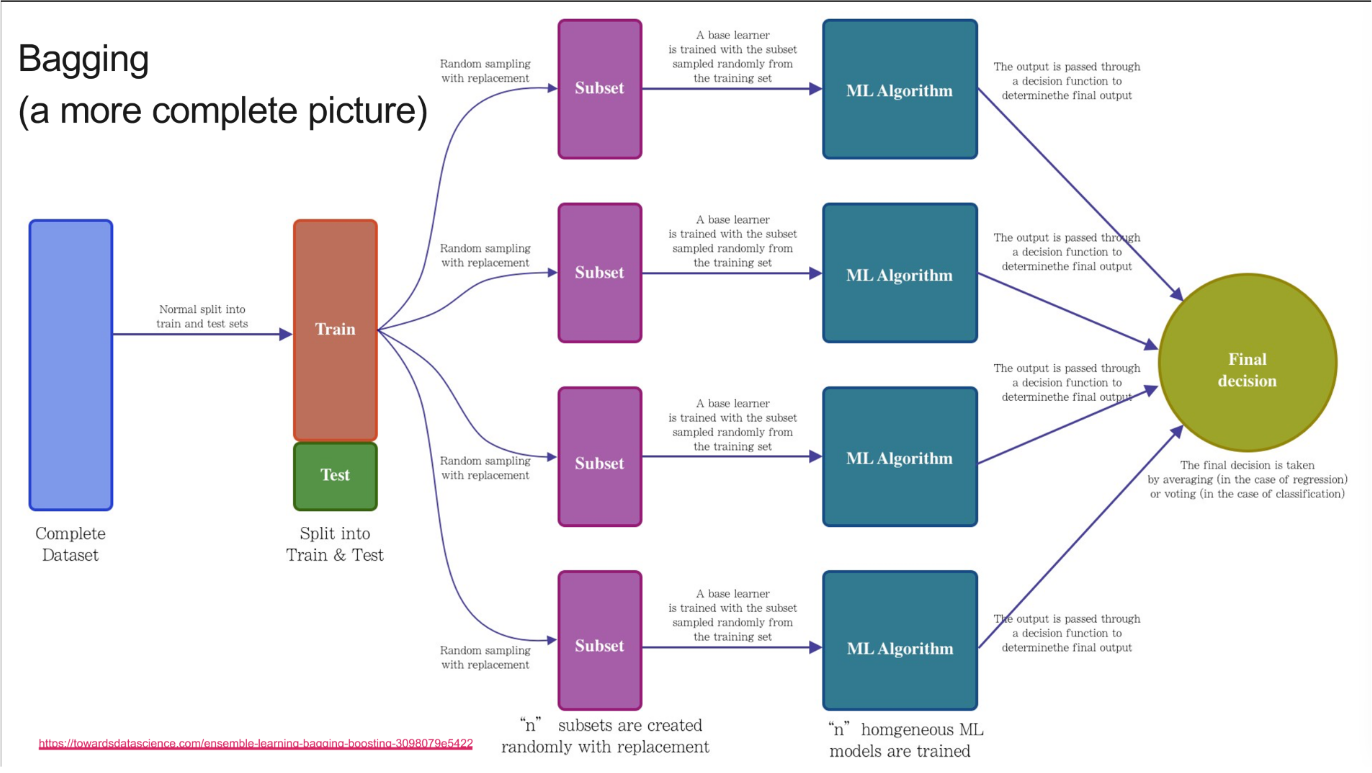
\includegraphics[width=\linewidth]{img/bagging_overview.png}
